\chapter{PROPOSTA DE SOLUÇÃO - WAFAMOLE++}
\label{chp:capitulo4}

Tendo em consideração o embasamento teórico estabelecido e a oportunidade de contribuir para um projeto de código aberto na área de interesse deste trabalho que tivesse abrangência e impacto, foi concebido o \textit{wafamole++} \footnote{Disponível no GitHub: https://github.com/nidnogg/wafamole-plusplus}, uma versão estendida do \textit{WAF-A-MoLE} anteriormente descrito no capítulo de Revisão de Literatura. Foram seguidas diretrizes e recomendações de contribuição estabelecidas pelos autores, e alguns módulos adicionais contendo funcionalidades não disponibilizadas pelos mesmos referentes ao treinamento de novos classificadores, geração de novos modelos, e tratamento de conjuntos de dados foram disponibilizados com este trabalho.

A elaboração do \textit{wafamole++} forçou um entendimento mais profundo da ferramenta original, recebendo apoio dos autores originais e atualmente conta com uma série de operadores de mutação novos e sobretudo modelos de classificadores novos implementados para um WAF de código aberto encontrado na plataforma de colaboração GitHub.

Acredita-se que essa colaboração contribuiu para tornar a ferramenta mais abrangente, com uma menor barreira de entrada para futuros colaboradores e mais flexível para avaliação de WAFs baseados em Aprendizado de Máquina no geral. Assim espera-se que mais contribuições possam ser geridas no futuro, estabelecendo-se como um projeto complementar ao \textit{WAF-A-MoLE} original.

\section{Visão Geral}
A introdução do \textit{wafamole++} como extensão do \textit{WAF-A-MoLE} é, sumariamente, uma versão do mesmo com uma série de módulos adicionais. O ambiente original carecia de uma documentação para as versões de suas dependências, e documentação de todas as suas etapas de treinamento, ocasionando em uma série de dificuldades para seu uso esperado. Além disso, havia espaço para adição de mais operadores de mutação e uma série de modelos diferentes que não foram inicialmente explorados pelos autores.

O \textit{wafamole++} resolve essas pendências introduzindo uma série de modelos e operadores de mutações novos, além de possuir uma documentação mais extensa (facilitando a instalação), com as etapas de treinamento transparentes o suficiente para que outros desenvolvedores possam replicá-las. Possui também como parte de suas extensões uma série de funções utilitárias para tratamento de dados, bastante importante para garantir a extensibilidade. 

\section{Arquitetura}

O \textit{wafamole++} possui uma estrutura composta de um classificador para realizar avaliações em cima dos dados trabalhados, uma interface em linha de comando para o usuário parametrizar seu funcionamento, e uma classe que realiza as técnicas de \textit{fuzzing} durante as rodadas de mutação.

Os operadores de mutação responsáveis por gerir as dadas iterações de \textit{fuzzing} ficam, idealmente, todos agrupados na classe \verb+SqlFuzzer+ dentro de seus métodos.

Diferentemente do \textit{WAF-A-MoLE} no entanto, a proposta inclui também um módulo separado responsável pelo tratamento, treinamento e geração de dados para alicerçar o funcionamento da aplicação principal. 

Uma representação visual da proposta, sem especificações como linguagens usadas, extensões de arquivo e detalhes mais profundos pode ser conferida no diagrama da Figura 8. Sua versão com maior nível de detalhamento é disponibilizada na Figura 10, mais adiante na Seção de implementação.

Descrevendo de forma geral essa estrutura, cada retângulo com título indica um módulo, seus subtítulos representam submódulos/métodos contidos nesses, e setas indicam ações ou comandos realizados por essas estruturas. Resumidamente, detalhando do topo da arquitetura até a base, tem-se:

\begin{alineas}
\item Um módulo \verb+Database+ - Nele se encontra um gerador de consultas \verb+mole_query_generator+ que executa o programa diversas vezes para acumular casos a serem adicionados na base de dados, um programa \verb+sqli_cleaner+ para tratamento de dados brutos e formatação para o WAF a ser testado, e os dados em si.

\item O MLBasedWafClassifier - Esse módulo responsável por receber os dados do módulo de \verb+Database+, estruturar o classificador do WAF \textit{MLBasedWAF} através de treinamento, gerar seu modelo correspondente e exportá-lo para uso na aplicação principal na parte de modelos.

\item Command Line Interface, ou Aplicação de linha de comando - Aqui é abrigada a típica função \textbf{main}, sendo aonde são recebidos os parâmetros a serem executados na aplicação pelo usuário como o número máximo de iterações, modelo a ser usado, e injeção SQL inicial para ser transformada em um exemplo adversarial. Esses parâmetros são explicados na Seção adiante.

\item Models - Aonde são armazenados os modelos. Modelos são classificadores de WAFs já treinados, exportados de forma que não seja necessário realizar o treinamento a cada iteração. 

\item EvasionEngine + SqlFuzzer - A classe \verb+EvasionEngine+ realiza cada iteração da aplicação que consiste em chamar a classe relacionada \verb+SqlFuzzer+ que transforma (via \textit{fuzzing}) a entrada inicial com os operadores de mutação nela contidos, armazenar a saída dessa transformação, e chamá-la novamente para obter uma transformação mais sofisticada. A condição de parada é fornecida pelo usuário, tanto na forma de iterações máximas, como na forma de uma \textit{threshold} máxima de confiabilidade (mais explicada na Seção adiante).

\end{alineas}

\begin{figure}[H]
    \centering
    \caption{Proposta wafamole++}
    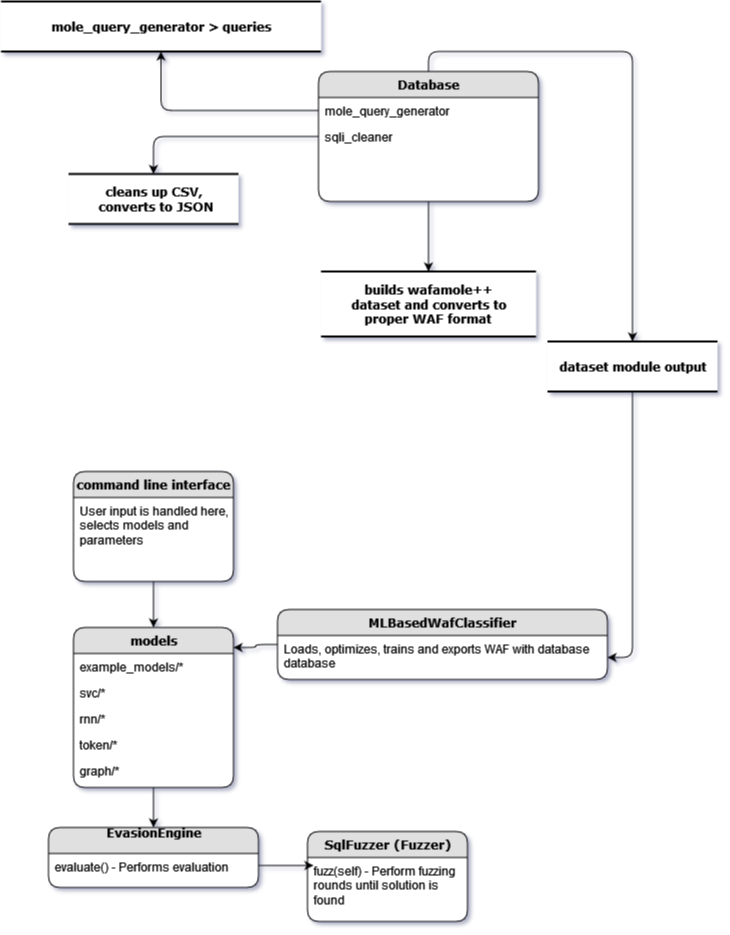
\includegraphics[width=16cm]{figuras/wafamole_proposal_language_agnostic.png} 
    \label{fig:internet} 
\end{figure}

\section{Implementação}

A solução foi implementada na linguagem \textit{Python} 3.8, seguindo as dependências encontradas nos arquivos intitulados \verb+requirements.txt+ no repositório final (disponível no GitHub \footnote{GitHub - Repositório Final: https://github.com/nidnogg/tcc}). O cerne do projeto encontra-se nos seguintes módulos:
\begin{alineas}
\item \verb+Main+ - Responsável pela lógica da linha de comando, com todos os decorators da biblioteca \verb+Click+ que facilitam o desenvolvimento de utilidades de terminal. Aqui é feito o recebimento e passagem de parâmetros para a pipeline do programa aqui, além de ser instanciada a classe principal \verb+wafamole+ e o módulo \verb+EvasionEngine+ com o modelo selecionado pelo usuário.
\item \verb+models+ - Em models estão localizados os modelos de exemplo para experimentação, modelos padrões do \textit{WAF-A-MoLE} e sobretudo modelos novos (também customizáveis) introduzidos no \textit{wafamole++}, localizados na pasta \verb+/models/svc+. Modelos novos de classificadores de WAFs a serem testados são tipicamente arquivos \verb+.dump+ das classes de tais classificadores, gerados através biblioteca \verb+joblib+ após o treinamento (no caso do \verb+scikit-learn+, da função \verb+.fit()+). Alternativamente, essa biblioteca permite também a geração de um arquivo \verb+.dump+ de uma pipeline caso o treinamento exija mais de uma etapa, como uma tokenização para possibilitar o treinamento de um dado classificador.
\item \verb+EvasionEngine+ - Essa classe contém o loop principal que requisita as mutações responsáveis pela transformação do \textit{payload} fornecido pelo usuário em um \textit{payload} considerado inócuo para o WAF sendo avaliado. As requisições são feitas ao módulo \verb+Fuzzer+.
\item \verb+Fuzzer+ - Nesse módulo ficam armazenados os operadores de mutação que transformam o \textit{payload} a cada rodada de mutação efetuada, sendo que cada mutação ocorre dentro do mesmo. Um operador de mutação dentre estes é escolhido aleatoriamente a cada iteração da pipeline principal.
\end{alineas}

Esses módulos, no entanto, não podem ser trivialmente estendidos sem alguns componentes auxiliares criados para o \textit{wafamole++}, que são:
\begin{alineas}
\item \verb+datasets+ - Aqui são contidos os conjuntos de dados SQLiV3, SQLiV4, e SQLiV5, funções de tratamento para os mesmos e uma função de geração/adaptação do conjunto de dados original do \textit{WAF-A-MoLE} para servir de treinamento para o MLBasedWAF, um WAF que será descrito na seção seguinte. O \verb+SQLiV3.json+ é o primeiro conjunto de dados utilizado para tal, disponibilizado pelo Kaggle \footnote{Kaggle - SQL Injection Dataset: https://www.kaggle.com/datasets/syedsaqlainhussain/sql-injection-dataset} \cite{kaggle_dataset_sql} e também está descrito adiante. Versões subsequentes (indicadas pelos números ascendentes) são incrementos realizados e testados nele com reforços de \textit{payloads} oriundos do wafamole++.

\begin{alineas}
\item \verb+mole+ - Essa função pode ser visualizada no Código 3 mais adiante. Ela executa em linha de comando o \textit{wafamole++} para cada linha do conjunto de dados SQLiV3, de modo a gerar um leque mais amplo de ataques. Como se trata de um processo iterativo, um limite superior de 7000 novos \textit{payloads} foi adotado - e o tempo de execução médio foi em torno de 8 horas para o processo todo. Para gerar novos ataques (dado que o \textit{wafamole++} produz saídas diferentes a cada execução), basta executá-lo com redireção de saída padrão (\verb+>+):
\begin{verbatim}
./mole_query_generator.py > output.json
\end{verbatim}


\item \verb+sqli_cleaner+ - Essa função auxiliar foi codificada inicialmente com a finalidade de transformar o conjunto de dados \verb+SQLiV3.json+ do formato .csv para .json que seria mais simples de trabalhar em \textit{Python}, além de adaptá-lo para o padrão visto no \textit{MLBasedWAF}. Essa função também contorna de uma série de inconsistências nos dados originais através de um polimento e tratamento de certos casos para que a saída do \textit{wafamole++} seja ideal. Seu código está disponível nessa seção, mais adiante no Código 8..

\item \verb+wafamole_dataset_generator+ - Fornecido apenas após um certo período de espera de alguns meses (compreendido entre a troca de emails com os autores originais), o conjunto de dados do \textit{WAF-A-MoLE} encontra-se disponibilizado no seu \href{https://github.com/zangobot/wafamole_dataset}{repositório}\footnote{GitHub - wafamole\_dataset: https://github.com/zangobot/wafamole_dataset} de maneira modular - com uma série de arquivos \verb+.json+ pequenos devido ao limite imposto pela plataforma GitHub. Além disso, ele precisou ser adaptado para o formato do \textit{MLBasedWAF} assim como o \verb+SQLiV3.json+ (sem dificuldades nesse caso). Possui uma abrangência e riqueza maior no geral do que o antecessor. Essa função realiza a combinação e adaptação das partes disponibilizadas pelos autores.

\end{alineas}
\item \verb+MLBasedWafClassifier+ - Localizada na pasta dos modelos customizados (models/svc), esse arquivo \textit{Jupyter Notebook} \footnote{Jupyter Notebook ou arquivo .ipynb: Um ambiente de desenvolvimento que permite organizar uma aplicação separando em pedaços de código e trechos de texto} é responsável por uma série de funções realizadas em cima dos conjuntos de dados baseados no \verb+SQLiV3.json+. É realizada a visualização dos dados contidos nos mesmos via gráficos, e os dados são agrupados de maneira a serem classificados para uso no \textit{wafamole++}. Dois tipos de classificadores são suportado Máquina de vetores de suporte não linear e Gradiente Descendente Estocástico. 

Um exemplo de um gráfico gerado pelo notebook com seu código correspondente pode ser encontrado na Figura 9.

\begin{figure}[ht]
    \centering
    \caption{Exemplo de gráfico gerado pelo Notebook}
    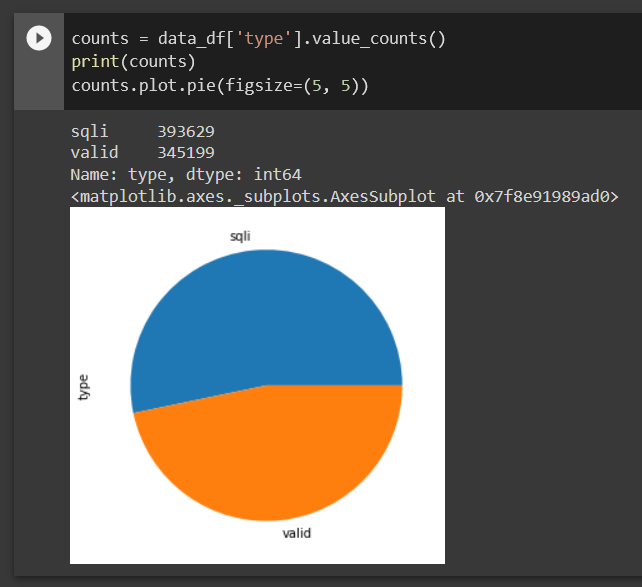
\includegraphics[width=16cm]{figuras/exemplo_grafico_notebook.png} 
    \label{fig:internet} 
\end{figure}

Para cada classificador é feita uma divisão em dados de treinamento e teste, para que seja averiguada a eficácia do modelo gerado ao fim da execução do código. Também é executada uma rotina \textit{GridSearchCV} para exaustivamente obter parâmetros mais otimizados para uso na classificação. Por fim, é chamada a função \verb+fit()+ responsável pela classificação, e o classificador resultante é testado. 

Os resultados desses testes sendo colocados em métricas como a matriz de confusão \footnote{Também conhecida como Matriz de Erro, essa matriz permite extrair uma série de métricas acerca da qualidade do modelo gerado, como taxas de falso positivo/negativo e verdadeiro positivo/negativo, além de acurácia e precisão.} e pontuação, e a biblioteca \textit{joblib} exporta um arquivo \verb+.dump+ com o modelo final para uso no \textit{wafamole++}. O final do componente contém testes com consultas SQL geradas pelo \textit{wafamole++} que penetram o WAF avaliado no notebook.

Para maior detalhamento e visualização das métricas no mesmo, o notebook está disponibilizado no \href{https://github.com/nidnogg/tcc}{repositório} final \footnote{GitHub - Implementação Final: https://github.com/nidnogg/tcc}, localizado sob a pasta \verb+models/custom/svc+.

\item \verb+MLClassifierWafamole+ - Trata-se de uma versão semelhante ao notebook anterior, porém fazendo uso do conjunto de dados original do wafamole, um banco consideravelmente mais robusto e amplo no geral. Por robustez, entende-se por consultas em maior numerosidade (uma diferença quase 690.000 registros a mais do que o conjunto de dados do Kaggle), e por amplitude, a variedade de comandos SQL nos registros, sendo mais representativo. 

O tamanho deste conjunto de dados exigiu algumas alterações para que os algoritmos rodassem apropriadamente, sendo um obstáculo no desenvolvimento do trabalho no geral, pois o processamento do mesmo exigia mais recursos, tempo e algumas modificações em eficiência para que funcionasse. Destaca-se aqui o uso do \textit{back-end} paralelo \verb+ray+ \cite{ray_backend_parallel} como considerável ganho de performance. Mesmo assim, algumas execuções foram realizadas por um período maior do que 48 horas e abandonadas sem resultados na etapa de treinamento.

No geral, este notebook possui um tempo de execução consideravelmente maior  em razão do conjunto de dados utilizado, o que é de se esperar e não pode ser evitado. Outra diferença chave são os classificadores usados - foram testados além dos dois anteriores o classificador \textit{AdaBoost}, com resultados promissores. A Máquina de vetores de suporte não linear, no entanto, não foi frutífera, requerendo um tempo de execução que excedia 48 horas. Cabe salientar que a versão mais recente desse notebook foi disponibilizada no \textit{Google Colab} sob o nome \verb+MLClassifierColabWafamole.ipynb+, via um link providenciado no repositório final.
\end{alineas}

De forma a ilustrar a implementação de uma maneira geral e como esses módulos se comunicam, a Figura 10 é disponibilizada, e para melhor detalhamento o componente \verb+mole+ pode ser visto no Código 3 por inteiro.

\label{sec:codigos}
\includecode[C]{Reforço de conjunto de dados SQLiV3.json do Kaggle} {alg:codigo2}{codigos/mole_query_generator.py}
\bigskip

Na Figura 10, as principais diferenças para a Figura 8 (que ilustra a arquitetura independente de tecnologias empregadas) se encontram no nome dos módulos, na extensão de arquivos e um detalhamento maior em módulos como \verb+datasets+ e \verb+cli.py+. Destaca-se dentre os detalhes os operadores da biblioteca \textit{Python} \verb+click+, que facilitam o uso do programa através da linha de comando (localizado no módulo \verb+cli.py+), o método \verb+evade()+ que é chamado na execução principal do programa e dá início ao funcionamento do mesmo, e uma melhor ilustração à direita de \verb+evasion.py+ de como o \textit{loop} principal de mutação é feito, com o método \verb+mutation_round()+.

Além desses detalhes, há uma bipartição no módulo de classificador, que se deu pela particularidade dos múltiplos conjuntos de dados que foram usados no \textit{wafamole++}. Acredita-se que em uma implementação nova, tendo acesso aos dados originais no início do desenvolvimento, não seria necessário explorar mais de um banco inicial de injeções e comandos SQL, apenas aprimorá-lo com mais entradas, fazendo uso do mesmo módulo de classificador caso desejado.

\begin{figure}[H]
    \centering
    \caption{Implementação do wafamole++}
    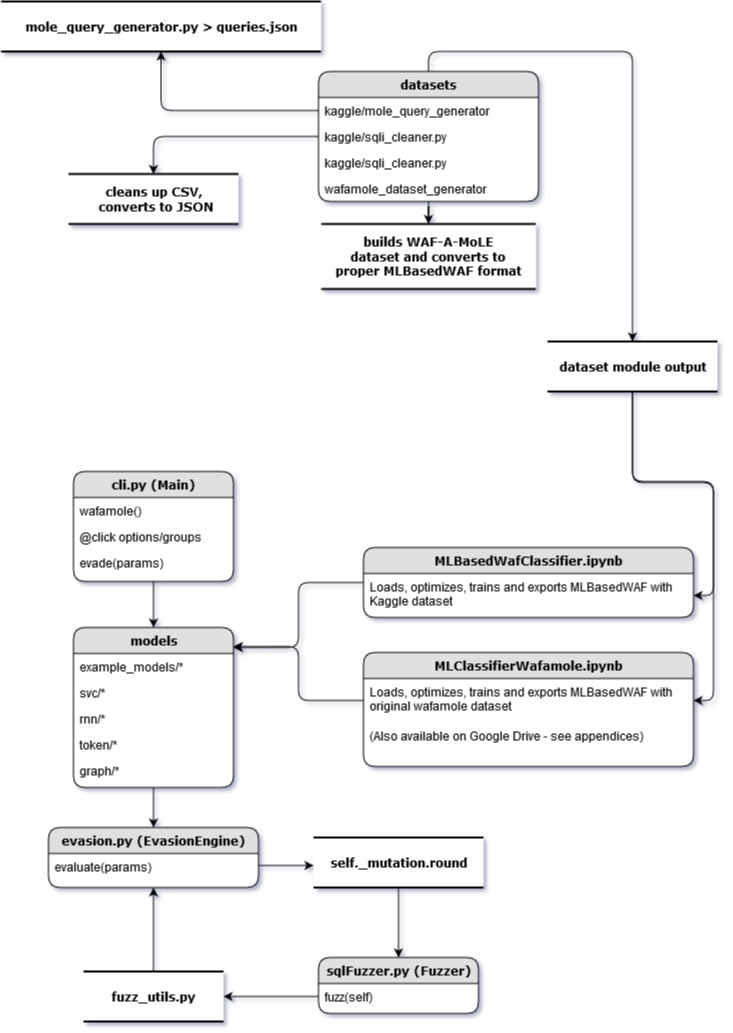
\includegraphics[width=16cm]{figuras/wafamole++_architecture.png} 
    \label{fig:internet} 
\end{figure}

\section{Operadores de Mutação}

O papel dos Operadores de Mutação tanto no \textit{WAF-A-MoLE} quanto no \textit{wafamole++} é fundamental, atuando como as ferramentas para guiar as mudanças realizadas no \textit{payload} atual a cada iteração do algoritmo. Sendo assim, considerando-se como o primeiro desenvolvimento feito na extensão do programa original, o \textit{wafamole++} conta com três novos operadores de mutação adicionados ao montante original. Todos estes encontram-se agrupados na classe \verb+sqlfuzzer.py+, localizada na pasta \textbf{payloadfuzzer} da aplicação.

A finalidade destes novos operadores é incrementar a variedade de exemplos adversariais gerados. O primeiro destes é o \verb+shuffle_integers+, mostrado no Código 4.

\label{sec:codigos}
\includecode[C]{Operador de mutação shuffle integers} {alg:codigo2}{codigos/operadores/shuffle_integers.py}

\bigskip

Sua implementação é a mais simples dentre os operadores novos - consistindo apenas na troca de números presentes no \textit{payload} atual que lidera a fila principal por números inteiros diferentes entre 0 e 9. Selecionam-se números no \textit{payload} (denominados de candidatos), a posição dos mesmos e seus conteúdos são armazenados e então uma substituição aleatória é escolhida e o \textit{payload} modificado é retornado.  

Interessantemente, modificando-se uma parte desse funcionamento para trocar a base numérica entre binário, octal, decimal e hexadecimal, obtém-se o próximo operador de mutação, com uma performance mais robusta. Trata-se do \verb+shuffle_bases+ (Código 5).

\label{sec:codigos}
\includecode[C]{Operador de mutação \textit{shuffle bases}} {alg:codigo3}{codigos/operadores/shuffle_bases.py}

\bigskip

Nessa função a seleção e armazenamento de posições a serem modificadas é virtualmente idêntico - porém a substituição conta com uma lista de modificações em potencial dentre as quais uma é amostrada aleatoriamente na hora de ser realizada a mutação. Também são considerados os casos em que a mutação não ocasiona em variações no \textit{payload} final. Finalmente, há o \verb+spaces_to_symbols+ - o operador com a performance mais interessante (Código 6).

\label{sec:codigos}
\includecode[C]{Operador de mutação spaces to symbols} {alg:codigo3}{codigos/operadores/spaces_to_symbols.py}

\bigskip

O operador \verb+spaces_to_symbols+ difere dos anteriores no que tange a posições que serão potencialmente modificadas - pois busca espaços em branco e não números. Com isso, a partir de uma lista gerada no algoritmo de símbolos como sinais de pontuação para substituição, um espaço é escolhido aleatoriamente e substituído por um desses símbolos.

\bigskip

\section{Modelos e WAFs avaliados}

Relembrando alguns conceitos vistos anteriormente, para melhor compreender essa seção é importante ter em mente que modelos, classificadores e WAFs estão relacionados da seguinte maneira: 

\begin{alineas}
\item Um determinado WAF baseado em Aprendizado de Máquina possui um classificador em seu funcionamento;
\item Um classificador deste WAF pode, após a etapa de treinamento de dados (que consome bastante tempo), ser "exportado" na forma de um modelo como um arquivo \verb+.dump+ ou \verb+.h5+ através da biblioteca \textit{Python} \verb+joblib+.
\end{alineas}

As seções a seguir podem então ser interpretadas da seguinte forma:
\begin{alineas}
\item \textbf{WAF-Brain} - Um WAF, cujo classificador após o treinamento é usado como modelo no \textit{wafamole++};
\item \textbf{SQLiGOT} - Mesma coisa que a seção anterior;
\item \textbf{MLBasedWAF} - Um WAF, cujo classificador foi treinado de diferentes formas e cada forma gerou um modelo diferente;
\item \textbf{Máquina de vetores de suporte} - Um modelo baseado no classificador do MLBasedWAF;
\item \textbf{Gradiente Descendente Estocástico} - Outro modelo baseado no classificador do MLBasedWAF;
\item \textbf{AdaBoost} - Outro modelo baseado no classificador do MLBasedWAF;
\item \textbf{Interface Scikit-Learn} - Uma classe que permite com que cada modelo \textit{scikit-learn} funcione no \textit{wafamole++}. Não é um modelo.
\end{alineas}
\subsection{WAF-Brain}

\textbf{Autores}: Sergio D Fdez, cr0hn, Enrique Garcia. Disponível no \href{https://github.com/BBVA/waf-brain}{GitHub}. \footnote{GitHub - waf-brain: https://github.com/BBVA/waf-brain}

O WAF-Brain \cite{waf_brain} foi um dos primeiros firewalls a serem testados pela equipe do \textit{WAF-A-MoLE}, e subsequentemente é o primeiro modelo de exemplo disponibilizado para testes na documentação do mesmo. Dessa maneira, foi testado com os novos operadores de mutação, sendo de ajuda para diagnosticar os incluídos no wafamole++. A Figura 11 é uma captura de tela do seu repositório, destacando a versão de \textit{Python} em que foi escrito, quantia de problemas abertos e logomarca.

\begin{figure}[ht]
    \centering
    \caption{Dependências e logomarca do WAF-Brain}
    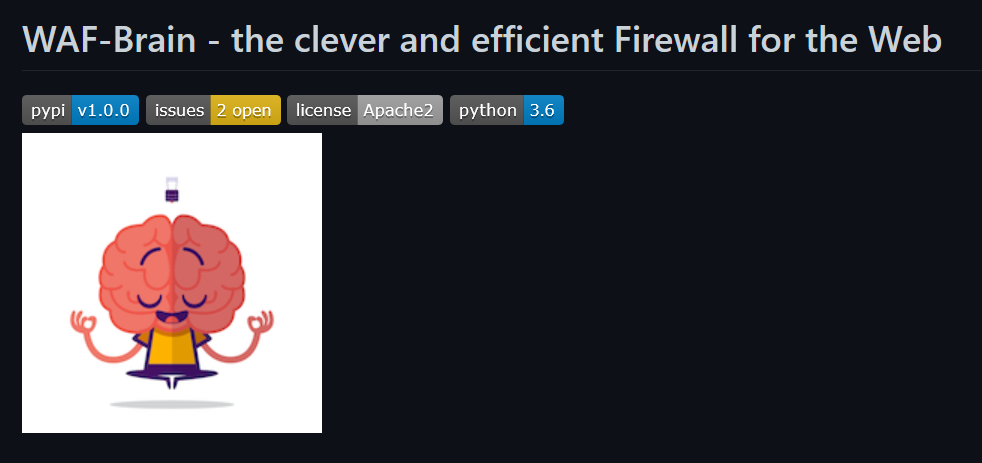
\includegraphics[width=12.5cm]{figuras/WAFBrain.png} 
    \legend{Fonte: \href{https://github.com/BBVA}{GitHub} (2019)}
    \label{fig:internet} 
\end{figure}

Seu funcionamento se dá, como anteriormente mencionado, através da estratégia de \textit{Deep Learning} com Redes Neurais, pela qual são analisados cada campo de um determinado pedido HTTP que passam pelo \textit{Firewall} sob a ótica de um classificador treinado desta maneira, determinando se esse campo é malicioso ou não. Caso haja um campo marcado como malicioso, o pedido HTTP é bloqueado.

Apenas o código \verb+inferring.py+ responsável pela análise de fato de um \textit{payload} do algoritmo é usado no \textit{WAF-A-MoLE} e \textit{wafamole++}. Nele há uma série de funções que preparam o conteúdo para ser avaliado pelo modelo treinado, como \verb+row_parse()+ (para pegar apenas caracteres definidos na constante \verb+VOCABULARY+, parametrizável pelo desenvolvedor), e \verb+reduce_dimension()+ (para adaptar as dimensões das frases analisadas em um \textit{array} da biblioteca \textit{numpy}).

Essas funções são utilizadas dentro da rotina \verb+process_payload()+, que realiza a chamada para o modelo através de \verb+model.evaluate()+ tendo como parâmetros os dados tratados pelas funções auxiliares anteriormente mencionadas. O resultado dessa função é efetivamente a probabilidade da entrada ser maliciosa ou não.

Na adaptação \textit{WAF-A-MoLE}, esse poder de predição é aproveitado exclusivamente na forma de probabilidade - tendo a probabilidade de ser uma injeção SQL acima de um determinado limite, temos um caso malicioso. Isso requer que o classificador treinado no modelo não apenas mostre a previsão como usualmente é feito, mas também a probabilidade de aquela previsão estar correta de fato.

Por mais que se trate de um algoritmo sofisticado por natureza, surpreendentemente o \textit{WAF-Brain} fora implementado pelos seus autores originais de uma maneira simplória o suficiente para ser um dos WAFs mais vulneráveis às estratégias de \textit{fuzzing} do \textit{WAF-A-MoLE}. Vários operadores de mutação isolados conseguem resultados frutíferos em pouco tempo, como será visto na seção de testes adiante.

\subsection{SQLiGoT}

\begin{citacao}[english]
BEFORE LAUNCHING EVALUATION ON SQLiGoT

These classifiers are more robust than the others, as the feature extraction phase produces vectors with a more complex structure, and all pre-trained classifiers have been strongly regularized. It may take hours for some variants to produce a payload that achieves evasion
\end{citacao}
\bigskip

Conforme essa advertência no \verb+README.md+ do repositório do \textit{WAF-A-MoLE} feita pelos autores, esse WAF exige um tempo de muitas horas (possivelmente além de um dia, verificado durante o trabalho) para ser penetrado pela aplicação. Além disso, seu código encontra-se inacessível, proibindo a experimentação para o escopo desse trabalho, impossibilitando até mesmo que sejam feitas as etapas de treinamento. Por esse motivo, o SQLiGOT \cite{kar2016sqligot} foi dispensado como alvo de estudo.

\subsection{MLBasedWAF}
Todos os modelos implementados tiveram como base o firewall ML-Based-WAF, disponível por vladan-stojnic no \href{https://github.com/vladan-stojnic/ML-based-WAF}{GitHub} \footnote{GitHub - ML-based-WAF: https://github.com/vladan-stojnic/ML-based-WAF} \cite{ml_based_waf} que fora o WAF de código aberto mais promissor e mais plausível de adaptar. Sua performance também era factível no contexto de recursos disponíveis para a conclusão deste projeto final, uma vez que não havia complexidade na arquitetura/implementação comparável a firewalls como o SQLiGOT \cite{kar2016sqligot}. Isso permitiu que os modelos resultantes pudessem ser executados tanto na plataforma Google Colab como localmente em alguns casos.

A Figura 12, retirada do repositório original desse WAF, mostra de forma geral a estrutura do MLBasedWAF. A pasta \textit{Classifier} contém alguns classificadores que são treinados com dados do conjunto de dados localizado na pasta \textit{Dataset}. Esses classificadores são replicados na pasta \textit{WAF} que contém as funcionalidades de um WAF propriamente dito, e o núcleo da aplicação.

Seu funcionamento se dá por uso de um \textit{script} (\verb+sniffing.py+, localizado na pasta \textit{WAF}) que vasculha tráfego real e/ou simulado de pacotes HTTP enviados à rede atual, que são então direcionados para um classificador baseado na biblioteca \textit{scikit-learn} que faz a predição se o pacote tem cabeçalhos maliciosos ou não. Esses cabeçalhos são agrupados entre benignos, ataques XSS, cmdi, e injeções SQL.

\begin{figure}[ht]
    \centering
    \caption{Repositório ML-Based-WAF}
    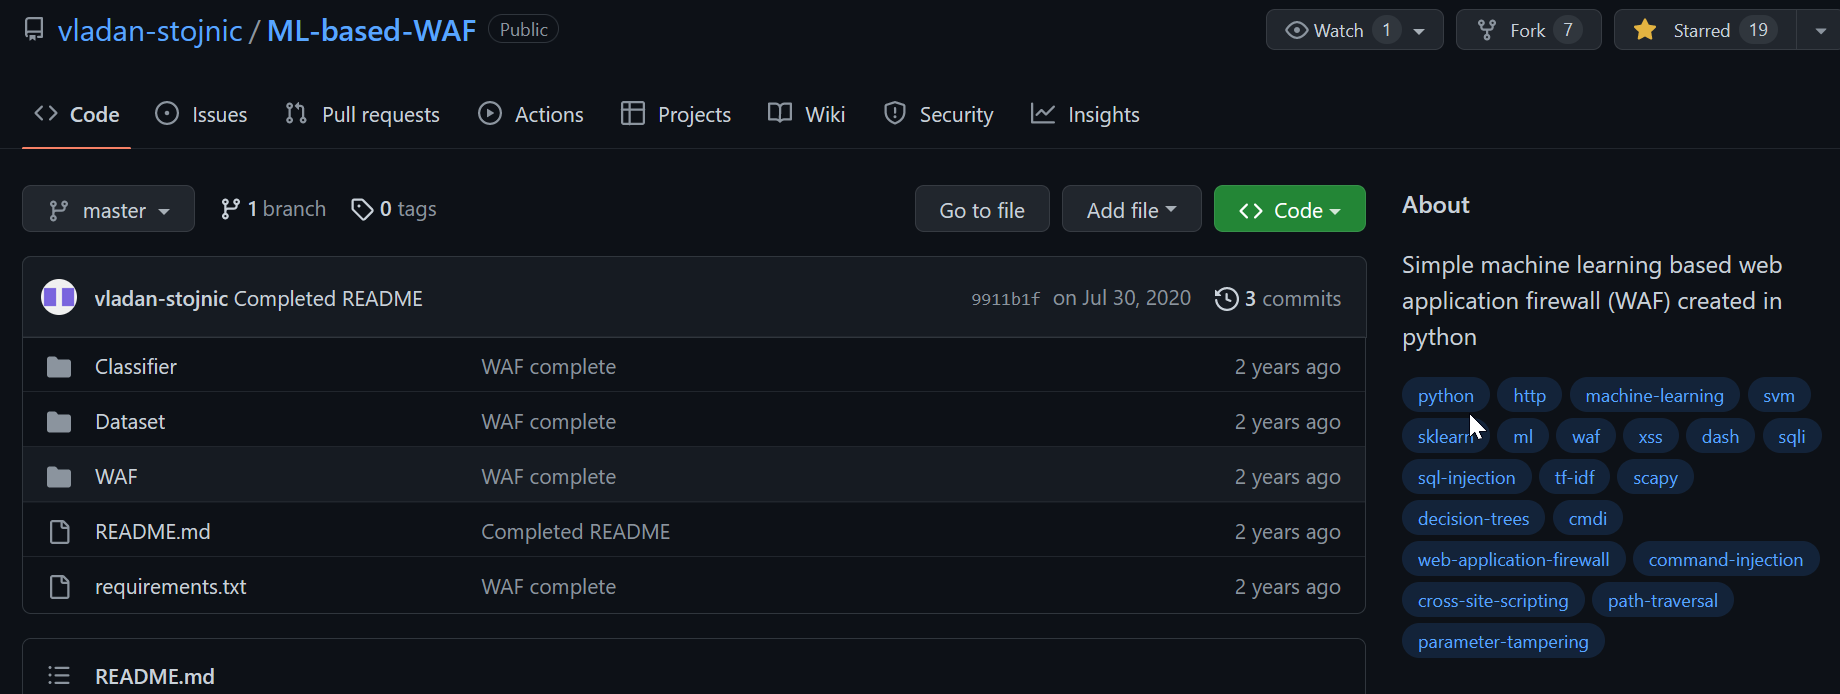
\includegraphics[width=16cm]{figuras/MLBasedWAF.png} 
    \legend{Fonte: \href{https://github.com/vladan-stojnic/ML-based-WAF}{GitHub} (2020)}
    \label{fig:internet} 
\end{figure}

Embora esse seja um WAF orientado ao tráfego real ou simulado de uma rede de fato, avaliando parâmetros HTTP em tempo real no seu componente \verb+sniffing.py+ tanto por injeções SQL como por outras formas de ataque (XSS, cmdi), ainda foi possível restringir seu funcionamento para adaptá-lo ao \textit{wafamole++} de forma que apenas injeções SQL fossem avaliadas, pois o \textit{WAF-A-MoLE} comporta apenas esse tipo de vulnerabilidade e o tempo de pesquisa e desenvolvimento para expandir para outros tipos não era viável para este trabalho.

Para tal, foi necessário prever uma estratégia própria de treinamento para o classificador, além de um conjunto de dados especial para o mesmo. É cabível mencionar, no entanto, que isso introduziu uma série de dificuldades uma vez que sua documentação era consideravelmente modesta, e o banco novo a ser usado deveria seguir o padrão de formatação seguido pelo WAF.

Dentre as opções de conjuntos de dados disponíveis com injeções SQL, foi escolhido inicialmente a versão \verb+SQLiV3.json+ da coleção do Kaggle \footnote{Kaggle - SQL Injection Dataset: https://www.kaggle.com/datasets/syedsaqlainhussain/sql-injection-dataset} \cite{kaggle_dataset_sql}, que foi anteriormente mencionada na seção de arquitetura do \textit{wafamole++}. A Figura 13 é uma captura de tela da página Web deste conjunto de dados, destacando alguns detalhes e metadados de relevância como número de valores únicos, categorias de dados, tamanho de arquivo e etc.

\begin{figure}[ht]
    \centering
    \caption{Detalhes conjunto de dados SQL Injection Kaggle.}
    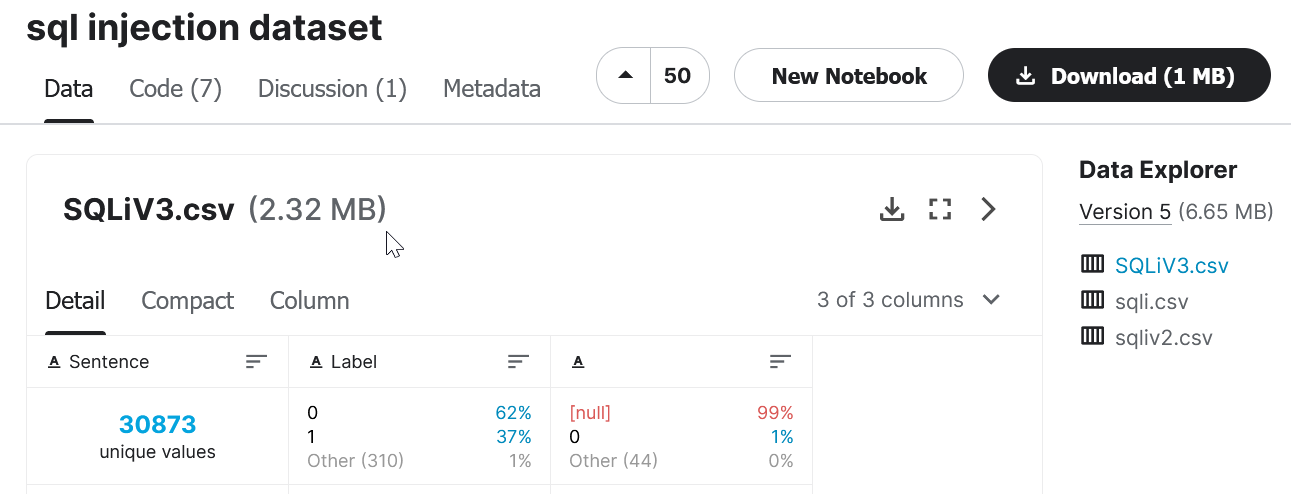
\includegraphics[width=16cm]{figuras/sqlInjectionDataset.png} 
    \legend{Fonte: \href{https://www.kaggle.com/datasets/syedsaqlainhussain/sql-injection-dataset}{Kaggle} (2021) https://www.kaggle.com/datasets/syedsaqlainhussain/sql-injection-dataset}
    \label{fig:internet} 
\end{figure}

A etapa de correção de uma variedade de erros de formatação, polimento de algumas consultas incorretas (e de difícil proveito), e adaptação para o padrão .json utilizado pelo WAF, encontra-se codificada na função auxiliar \verb+sqli_cleaner.py+, no Código 7.


\label{sec:codigos:sqli_cleaner}
\includecode[C]{Para tratamento de dados brutos} {alg:codigo3}{codigos/sqli_cleaner.py}
\bigskip


\subsection{Máquina de vetores de suporte}
Este foi o primeiro modelo implementado no \textit{wafamole++}, antes do recebimento do conjunto de dados original da equipe dos autores. Foi executado no módulo do conjunto de dados do Kaggle e no módulo do conjunto de dados original do \textit{WAF-A-MoLE}. Dado isso, esse classificador foi implementado com êxito apenas usando os conjuntos de dados \verb+SQLiV3.json+, \verb+SQLiV4.json+ e \verb+SQLiV5.json+. Tais conjuntos de dados correspondem, respectivamente, aos seguintes modelos:
\begin{alineas}
\item \verb+test_svc_classifier_no_mole.dump+

(equivalente ao \verb+svc_trained.dump+);
\item \verb+test_svc_classifier_moled.dump+;
\item \verb+test_svc_classifier_extra_moled.dump+ 
\end{alineas}

A nomenclatura \textit{moled} foi escolhida para mensurar o quão reforçado o conjunto de dados usado no treinamento é - sendo tal reforço definido como a quantia de consultas "fuzzeadas" pelo \textit{wafamole++} acrescentadas ao conjunto de dados inicial. E é evidente uma diferença na performance de cada modelo gerado - observou-se uma progressão de aumento (em média) de rodadas mutacionais (consumidas durante a execução) para os dois últimos modelos, especialmente no último.

Em termos de implementação, como fora usado no \verb+SVCClassifierWrapper+ criado em torno do \textbf{ML-Based-WAF} que usa a biblioteca \verb+scikit-learn+, esse modelo também a utiliza no seu funcionamento. O classificador usado no modelo é o \verb+SVC()+, definido como uma classe e trazido através de um comando de \verb+import+ - \verb+from sklearn.svm import SVC+. Essa classe é instanciada na pipeline \verb+make_pipeline+ (\verb+joblib+) com os parâmetros encontrados através de experimentação e otimização via \verb+GridSearch+ (uma espécie de força bruta para testar várias combinações de parâmetros e seus resultados subsequentes, explorado também no Capítulo 2). 

A divisão entre dados de validação e de teste é de 25\% do conjunto de treinamento como dados de teste, sem uso do algoritmo de \textit{K-fold} para a divisão (usando-se apenas o método da biblioteca \textit{scikit-learn} \verb+train_test_split()+).

Antes de fornecer os dados ao classificador \verb+SVC()+, os comandos SQL do conjunto de dados de entrada passam por uma etapa comum a todos os novos modelos, em virtude do funcionamento do \textbf{ML-Based-WAF} - uma vetorização através da classe \verb+TfidfVectorizer+, com os parâmetros padrões do WAF. Não foram feitos experimentos acerca dos parâmetros dessa classe intermediária. Isso divide os dados brutos, agrupando-os por palavras organizadas por seu peso em relação a entrada inteira, na forma vetores de rótulos (em inglês: \textit{feature vectors}) que serão lidos pelo classificador. Uma das vantagens de trabalhar com as pipelines da biblioteca \verb+joblib+ é poder usar a saída do vetorizador \verb+TfidfVectorizer+ como entrada da classe \verb+SVC()+ nela com facilidade, como ilustrado no Código 8.

Ao treinar um SVM com kernel RBF (\textit{Radial Basic Function}) que corresponde ao classificador não linear (discutido no Capítulo 2) existem dois parâmetros a serem considerados: \textbf{C} (que não é exclusivo do kernel RBF) e \textbf{Gamma}.

C faz uma troca entre classificar erroneamente durante os treinamentos e ter uma superfície de decisão \footnote{Existe uma representação visual bidimensional para classificação de aprendizado denominada superfície de decisão, onde as características que o classificador pode escolher são espaços delineados e as decisões são pontos dentro desses espaços.} mais simples. Um C baixo permite uma superfície de decisão suave, enquanto um C alto caminha para classificar os exemplos de teste corretamente. 

Já Gamma determina o quanto apenas um teste irá influenciar. Quanto maior o Gamma, mais próximos os outros valores precisam estar do teste para serem influenciados.

Valores de C e Gamma devidamente calibrados são críticos para a performance do SVM. Dado isso, os parâmetros utilizados para o classificador \verb+SVC()+ foram:
\begin{alineas}
    \item C (Parâmetro de Regularização - potência da regularização sendo o inverso proporcional a C): \textbf{10} 
    \item kernel (Tipo de kernel usado no classificador): \textbf{rbf};
    \item probability (Para fazer uso da métrica de probabilidade): \textbf{true};
    \item gamma (Coeficiente para o kernel escolhido): \textbf{scale}
\end{alineas}

\bigskip

Infelizmente um dos pontos de dificuldades foi o treinamento de um classificador deste tipo para o conjunto de dados original do \textit{WAF-A-MoLE}, recebido após os testes iniciais. Em suma, tempos de execução excederam 48 horas em alguns casos, impossibilitando a conclusão da função \verb+fit+ de treinamento, mesmo fazendo uso do backend de paralelização \verb+ray+.  Isso revelou uma inadequação do SVM para esse caso, sugerindo que outros classificadores sejam usados em seu lugar para conjuntos grandes de dados desse tipo.

Resumidamente, com isso tem-se que além da testagem em cima do reforço via \textit{wafamole++}, estruturalmente buscou-se diferenciar a implementação de Máquina de vetores de suporte da utilizada anteriormente no \textit{WAF-A-MoLE}. Diversos parâmetros foram modificados, e fazendo-se uso de uma busca \textit{paramgrid} (para testar exaustivamente combinações de parâmetros) complementada de experimentação após sua execução, foi possível obter essa configuração vista acima. 

Nesse contexto destaca-se um que troca o algoritmo fundamental por trás da Máquina de vetores de suporte por um com abordagem não linear (no caso, de parâmetro \verb+kernel = 'rbf'+) em contraste com o algoritmo linear empregado no modelo baseado em \textit{tokens} (intitulado simplesmente de \textit{Token-based}) padrão do WAF-A-MoLE. Isso permitiu resultados comparáveis aos originais (e, após reforço, com performance superior como indicado no Capítulo 5 adiante) com um classificador fundamentalmente diferente na mesma arquitetura, expandindo o leque de classificadores suportados na aplicação. Sua escolha foi impulsionada pela experimentação e a rotina \textit{GridSearchCV} de otimização de parâmetros.

Por fim, sua célula de código principal contida no \textit{Python} Notebook pode ser vista no Código 8.

\label{sec:codigos:modelos}
\includecode[C]{Pipeline classificador SVC Não-Linear}{alg:codigo3}{codigos/modelos/svc_model_sqliv3.py}
\bigskip

\subsection{Gradiente Descendente Estocástico}
O segundo modelo a ser programado pôde ser testado tanto para os conjuntos de dados do Kaggle como do \textit{WAF-A-MoLE} original, sem problemas de performance. No caso posterior, de fato houve uma exigência maior da máquina, requerendo um ambiente com mais memória que o desktop originalmente usado para executar os notebooks. Com isso, foi empregada a plataforma Google Colaboratory, da subdivisão de pesquisa da Google. 

Como no modelo anterior e nos subsequentes, sua implementação é realizada a partir de um comando \verb+import+ (\verb+from sklearn.linear_model import SGDClassifier+) da biblioteca \verb+scikit-learn+ e o classificador é instanciado na função \verb+make_pipeline()+. Uma diferença na sua implementação é que, como fora gerado um modelo para o conjunto de dados \textit{WAF-A-MoLE} também, este possui alguns pequenos ajustes no tratamento dos dados que servem de entrada para o treinamento. Os dados passam também pela etapa intermediária de vetorização através da classe \verb+TfidfVectorizer()+, conforme funcionamento do \textit{ML-Based-WAF}. 

A divisão entre dados de validação e teste é a comum a todos os modelos novos: de 25\% do conjunto de treinamento como dados de teste, sem uso do algoritmo de \textit{K-fold} para a divisão (usando-se apenas o método da biblioteca \textit{scikit-learn} \verb+train_test_split()+).

Para melhor compreender os parâmetros utilizados, \textbf{loss} é uma função para cálculo de perda do gradiente descendente estocástico a cada amostra em uma unidade de tempo. O parâmetro \textbf{penalty} tambem chamado de \textit{regularization} é uma penalidade adicionada à função \textbf{loss} que reduz os parâmetros do modelo em direção ao vetor zero. Por fim, \textbf{max\_iter} é o parâmetro que controla o número máximo de iterações durante o treinamento de dados, variando de 1 a infinito. Os valores utilizados no treinamento foram:
\begin{alineas}
    \item loss (Função de \textit{loss} - apenas essa retorna as estimativas de probabilidade necessárias): \textbf{modified\_huber};
    \item penalty (Também conhecido como termo de regularização. Valores como l1 aumentam esparsidade dos dados, não necessário nesse caso): \textbf{l2};
    \item max\_iter (Número máximo de "épocas" ou passadas sobre os dados de treinamento): \textbf{500}
\end{alineas}


A mudança de ambiente de notebooks localmente armazenados para o notebooks na plataforma Google Colaboratory ocasionou em uma série de vantagens, dentre as quais destacam-se: uma facilidade em executar um ambiente funcional, disponibilização de um link compartilhável, colaboração simultânea e principalmente mais memória RAM para executar as pipelines de treinamento. 

Um fator indesejável é a impossibilidade de gerenciar com maior precisão a versão de Python e algumas dependências - ocasionando numa séria poluição de logs em virtude da deprecação de algumas técnicas empregadas em versões antigas dos pacotes \verb+numpy+, \verb+scikit-learn+ e \verb+tensorflow+, dificultando o desenvolvimento e diagnóstico de erros. 

Acredita-se que a principal falha da plataforma, no entanto, seja a limitação de sua versão gratuita, no entanto, que desliga todas as células \footnote{Uma célula em um Jupyter Notebook é um pedaço qualquer do programa que pode ser ou um trecho de código em Python, ou um trecho escrito na linguagem de markup Markdown. Jupyter Notebooks são compostos inteiramente de tais células.} do Notebook em uso após um período fixo de 12 horas, a menos que o usuário esteja ativamente codificando na mesma. Isso dificultou o modelo discutido anteriormente, cujo fluxo de execução excedia facilmente esse intervalo para conjuntos de dados suficientemente grandes.

Não obstante, no caso do Gradiente Descendente Estocástico a performance foi satisfatória o suficiente para gerar um par de modelos a serem testados: um para o conjunto de dados \verb+SQLiV5.json+, intitulado de \verb+test_sgd_wafamole.dump+ (cujos parâmetros podem ser vistos no Código 9, na etapa antes de seu treinamento) e um para o conjunto de dados do \textit{WAF-A-MoLE}, \verb+sgd_trained.dump+. A performance dos mesmos será comparada mais detalhadamente no capítulo de testes adiante. 

\label{sec:codigos:modelos}
\includecode[C]{Pipeline classificador SGD sem backend de paralelização ray (Para SQLiV5.json)}{alg:codigo3}{codigos/modelos/sgd_model_sqliv3.py}
\bigskip

\subsection{AdaBoost}

O último modelo, e um dos mais interessantes, é o do classificador AdaBoost, implementado apenas para o conjunto de dados do \textit{WAF-A-MoLE} no final da implementação do trabalho. Sua performance é promissora, superando alguns dos modelos padrões do \textit{WAF-A-MoLE} como alguns dos baseados em Token e o WAF-Brain. Para treiná-lo, foi necessário o uso do backend de paralelização \verb+ray+, tomando ainda um tempo considerável de vários minutos. Sua respectivo \verb+import+ é do módulo \verb+ensemble+ do \verb+scikit-learn+, com o comando \verb+from sklearn.ensemble import AdaBoostClassifier+. Novamente, os dados passam pela etapa intermediária de vetorização através da classe \verb+TfidfVectorizer()+, conforme funcionamento do \textit{ML-Based-WAF}. 

A divisão entre dados de validação e teste é a comum a todos os modelos novos: de 25\% do conjunto de treinamento como dados de teste, sem uso do algoritmo de \textit{K-fold} para a divisão (usando-se apenas o método da biblioteca \textit{scikit-learn} \verb+train_test_split()+).

Os parâmetros deste classificador, por sua vez, precisam de ajustes pequenos:
\begin{alineas}
\item n\_estimators (Número máximo de estimadores que dita quando o \textit{boosting} \footnote{Boosting é o algoritmo que transforma um processo de aprendizado fraco em um de aprendizado forte e é melhor detalhado na Subseção 2.4.3, do Capítulo 2. Isso reduz viés e variância em aprendizado supervisionado.} é finalizado): \textbf{100};
\item random\_state (Controla uma \textit{seed} aleatória dada a cada \verb+base_estimator+ em iterações de \textit{boosting}. Com um inteiro nesse parâmetro, obtêm-se uma saída reproduzível em múltiplas chamadas a funções): \textbf{0}
\end{alineas}


O resultado desse modelo é intitulado de \verb+test_ada_classifier.dump+. No Código 10 é demonstrado e comentado com mais detalhes como é feita essa adaptação além da etapa de treinamento (note os métodos \verb+pipe.fit()+ e \verb+pipe.score()+, responsáveis pelo treinamento e avaliação respectivamente).

\label{sec:codigos:modelos}
\includecode[C]{Pipeline classificador AdaBoost com backend de paralelização ray}{alg:codigo3}{codigos/modelos/ada_model.py}
\bigskip

\subsection{Interface Scikit-Learn}
Por fim, para cada um desses novos modelos funcione, é necessária a criação de uma classe intitulada de \textit{SVCClassifierWrapper} (pois foi inicialmente criada com o SVC/SVM em mente, mas depois foi utilizada nos demais modelos criados) para servir de ponte entre a pipeline gerada pela biblioteca \verb+joblib+ (arquivos \verb+.dump+) e o \textit{wafamole++}. Relembrando a arquitetura do \textit{WAF-A-MoLE} original na Figura 6, essa classe seria o componente \verb+WAF Adapter+, porém um pouco mais abrangente servindo para qualquer classificador da biblioteca  \verb+sciki-learn+.

A classe encontra-se disponibilizada no Código 11 a seguir. É composta por dois métodos, \verb+classify()+ e \verb+extract_features()+. O método \verb+classify()+ é responsável por realizar a predição em si, e classificar uma entrada em maliciosa ou não. Essa classificação é expressa na forma de uma probabilidade da sua entrada ser maliciosa, e é desse formato que sai a necessidade de todos os classificadores implementarem o método \verb+predict_proba()+ anteriormente discutido no detalhamento dos parâmetros. 

Já o método \verb+extract_features()+ atua como uma simples função identidade, sendo usado dentro do método \verb+classify()+ também para verificação se as entradas usadas na classe são do tipo \verb+String+ ou não.

\label{sec:codigos:modelos}
\includecode[C]{Classe SVCClassifierWrapper para modelos novos}{alg:codigo3}{codigos/modelos/svc_wrapper.py}
\bigskip



